\documentclass{article}
\usepackage[utf8]{inputenc}
\usepackage{graphicx, graphics, float}
\usepackage[a4paper, total={6in, 9in}]{geometry}
\usepackage[spanish]{babel}
\title{Haz Una Línea\\
\large Memoria DS - Práctica 2}
\author{Andrés Merlo Trujillo\\ Sergio Hervás Cobo\\ Javier Serrano Lucas\\ Ricardo Molina Rodríguez}

\begin{document}
\date{Abril 2022}
\maketitle
\section{Introducción}
En esta práctica hemos decidido realizar con Flutter y Dart un videojuego de móvil
semejante al conocido ``Tetris'' con algunas funcionalidades y modificaciones adicionales
que hemos inventado para darle una mayor jugabilidad.

A continuación se describirá la funcionalidad de la aplicación así como los Requisitos
funcionales y no funcionales para su correcta comprensión:

\section{Descripción del sistema}
Para realizar la aplicación se ha utilizado el patrón de diseño creacional
 ``Factoría Abstracta'' junto con el de ``Prototipo''.\\

En la parte de creación de las piezas, que se realiza en la Factoría, hemos
 decidido usar el algoritmo que utilizan la mayoría de juegos de este tipo que
 consiste en idear un ``saco'' con las 7 piezas del juego. De este, se escoge una pieza al azar,
 causando así que haya una menos dentro. Posteriormente, de las piezas restantes se coge otra al azar
  y así sucesivamente hasta que no queden piezas. Cuando no queden piezas en el saco se vuelve
  a llenar con otras 7 piezas nuevas, todas distintas.

La ventaja de usar este algoritmo en vez de haber usado uno aleatorio puro es
 que el reparto de piezas distintas es uniforme, a diferencia de aleatorio puro
 que podía darse el caso de que saliera varias veces la misma pieza causando una
 mala experiencia para el jugador.\\

El tablero consta de una matriz de 20x10, donde van cayendo piezas sucesivamente
hasta que el tablero tenga bloques que lleguen hasta arriba del todo y no haya
opción de poder bajar la pieza siguiente dentro de los límites del tablero, en
ese caso será el GameOver. Para superar el juego tendremos que colocar
las piezas que van bajando de manera periódica alineando sus bloques mediante
giros y movimientos laterales para realizar una línea (o varias) horizontal de
10 bloques consecutivos. La linea completada desaparecerá del tablero y cada 10 líneas
completadas, el nivel de dificultad aumentará provocando un aumento de la velocidad de
bajada de la pieza y de la música del juego, causando un mayor reto al jugador.\\

Cabe destacar la implementación de la sombra de las piezas, que representan el lugar
donde van a caer. Esto es útil para poder guiar al usuario indicándole la posición
en la que se encontraría la pieza en caso de dejar la posición actual definitivamente.\\

Para determinar si ha caído o no tendremos que detectar una colisión con otra pieza
 o con el suelo del tablero y en cuanto ocurra, se añaden los bloques de la pieza
 al tablero y se escoge la siguiente del saco.\\

También se mostrará en pantalla la pieza reservada actual y las 3 piezas
siguientes para poder realizar mejores estrategias al jugar; además de una
sección que indica el nivel de dificultad, la puntuación y el número de líneas
completadas.\\

Por último, se ha realizado un modo de juego nuevo para darle más sentido a los
patrones que hemos escogido. Este modo consta de las siguientes características:

\begin{itemize}
\item Existirán piezas bomba que causarán la eliminación de todos los bloques a su alrededor,
incluyendo los de las esquinas y los de la propia pieza bomba. Estas piezas tendrán la misma forma
que las piezas normales, pero un color más oscuro para poder diferenciarlas.\\
Este tipo de piezas puede ser un arma de doble filo, pues por una parte te ayuda
 a eliminar bloques molestos mientras que por otro lado puede llegar a ser
 contraproducente al eliminar bloques que estaban en filas a punto de ser completadas.
\item Habrá una pieza '+' que dificultará la partida al jugador por su forma.
\end{itemize}


\subsection{Requisitos funcionales}
\begin{itemize}
    \item El sistema debe permitir pausar la partida en cualquier
    momento.
    \item El sistema debe permitir al usuario manejar el movimiento de
    las piezas (traslación y rotación)
    \item El sistema debe permitir al usuario reservar una pieza
    \item El sistema debe permitir iniciar la partida.
    \item El sistema debe mostrar una lista de piezas siguientes.
    \item El sistema debe mostrar la puntuación, el nivel y las filas por cada pieza puesta.
    \item El usuario podrá controlar la música tanto en volumen (subir o bajar) como en reproducción (pararla o reanudarla)
\end{itemize}
\subsection{Requisitos no funcionales}
\begin{itemize}
    \item El sistema debe trabajar en tiempo real para evitar inconsistencias.
    \item El sistema tendrá una interfaz para el menú para elegir modos y comenzar la partida.
    \item Las físicas del sistema no deben estar unidas a los fotogramas por segundo (FPS).
    \item Existirá un modo oscuro que cambie los colores de la interfaz


\end{itemize}
\subsection{Diagramas del sistema}
\begin{figure}[H]
        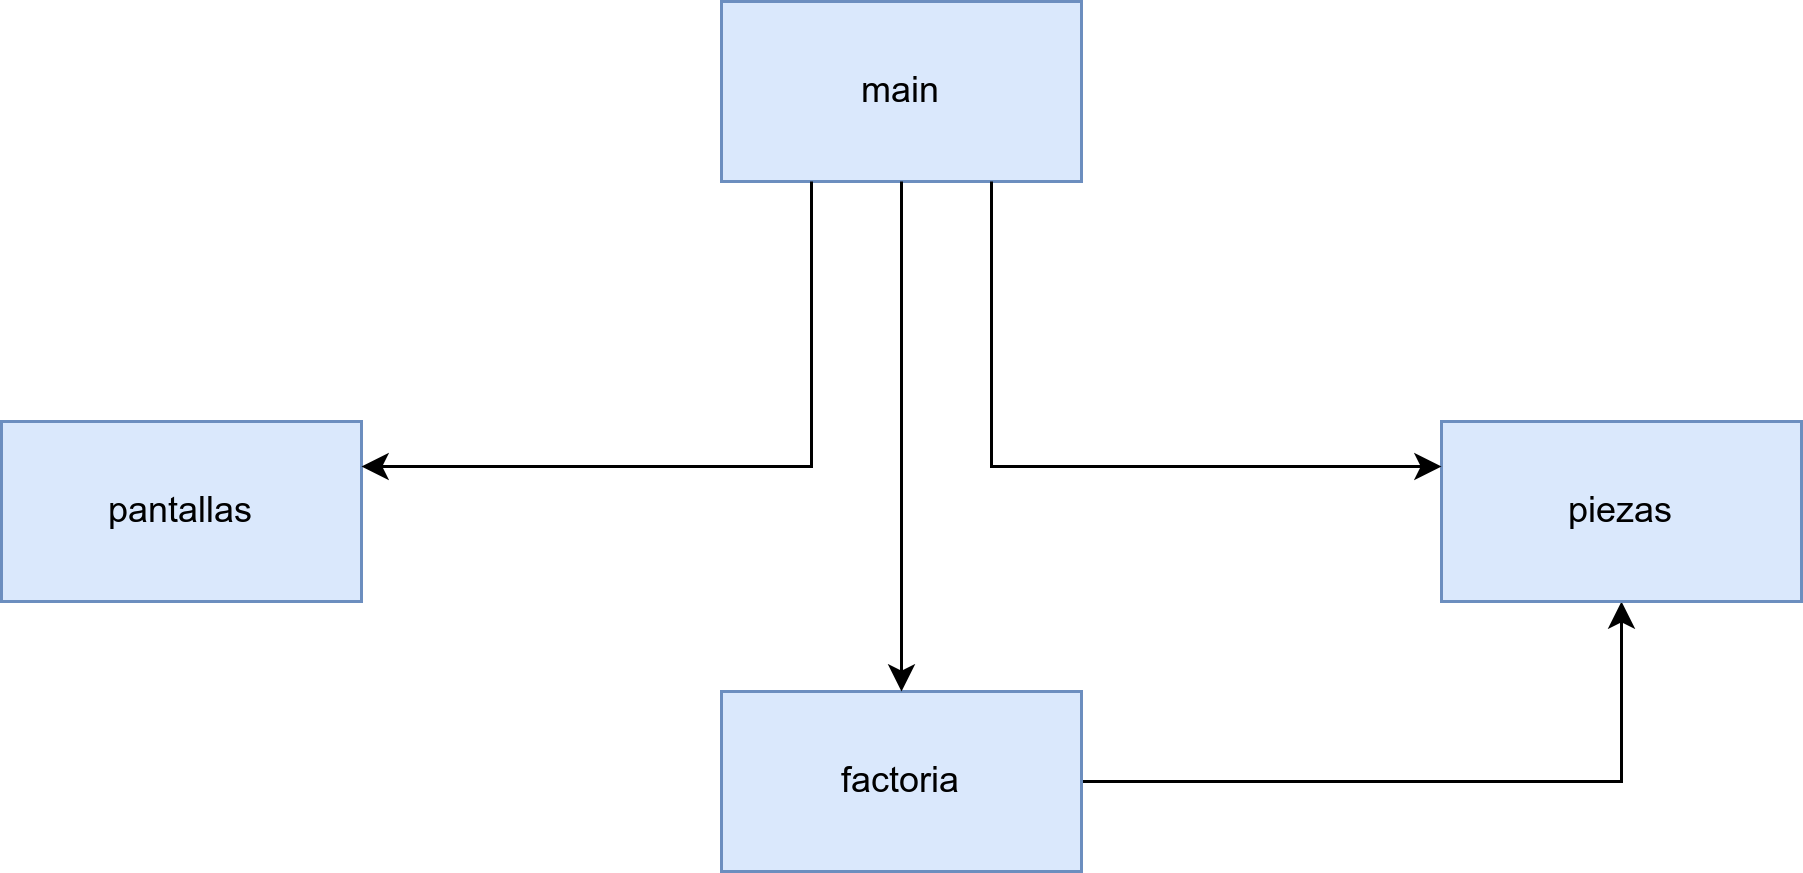
\includegraphics[width=\textwidth]{imagenes/paquetes.png}
        \caption{Diagrama de paquetes}
\end{figure}

\begin{figure}[H]
        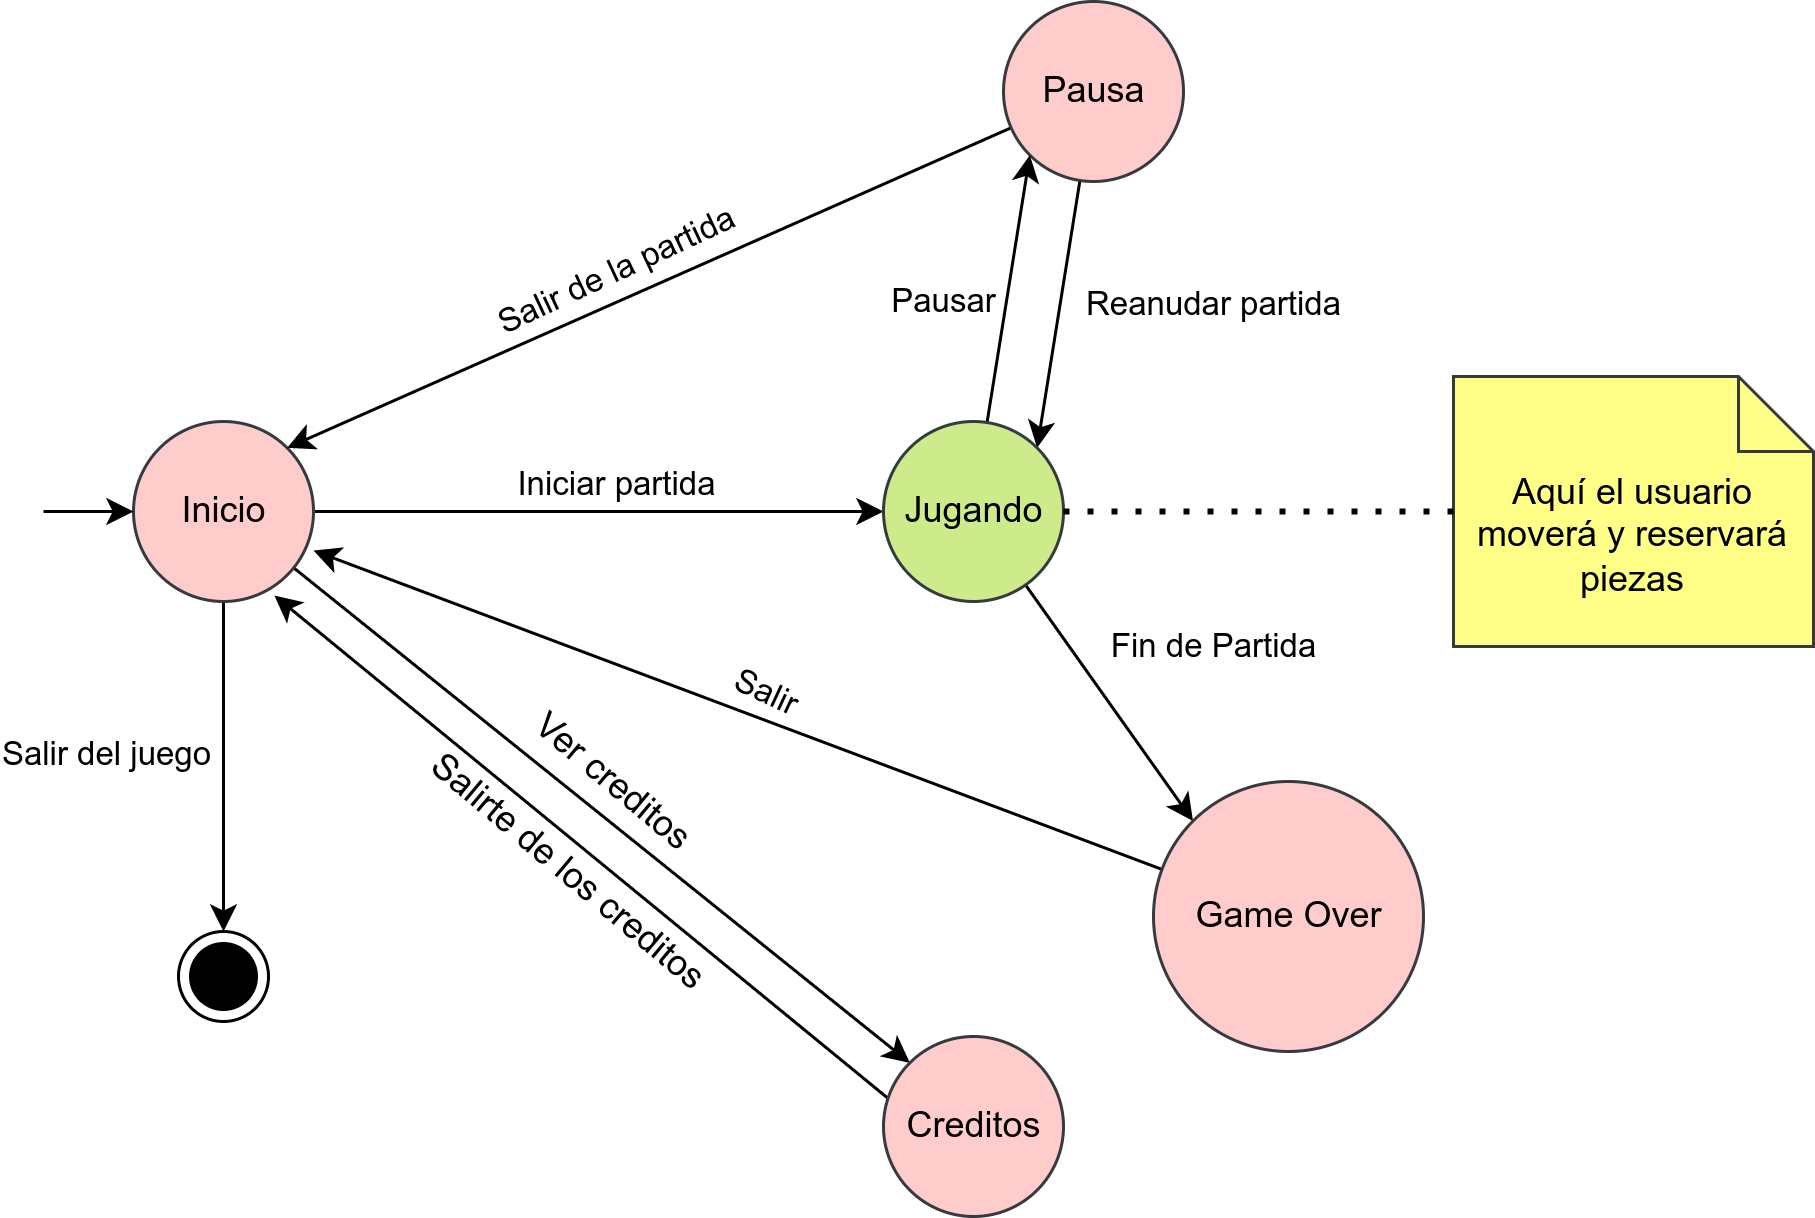
\includegraphics[width=\textwidth]{imagenes/estados.png}
        \caption{Diagrama de estados (autómata)}
\end{figure}

\subsection{Diagrama de clases}
\begin{figure}[H]
        \includegraphics[width=\textwidth]{imagenes/clase.png}
        \caption{Diagrama de clases}
\end{figure}

\section{Capturas de pantalla}
\begin{figure}[H]
\center
        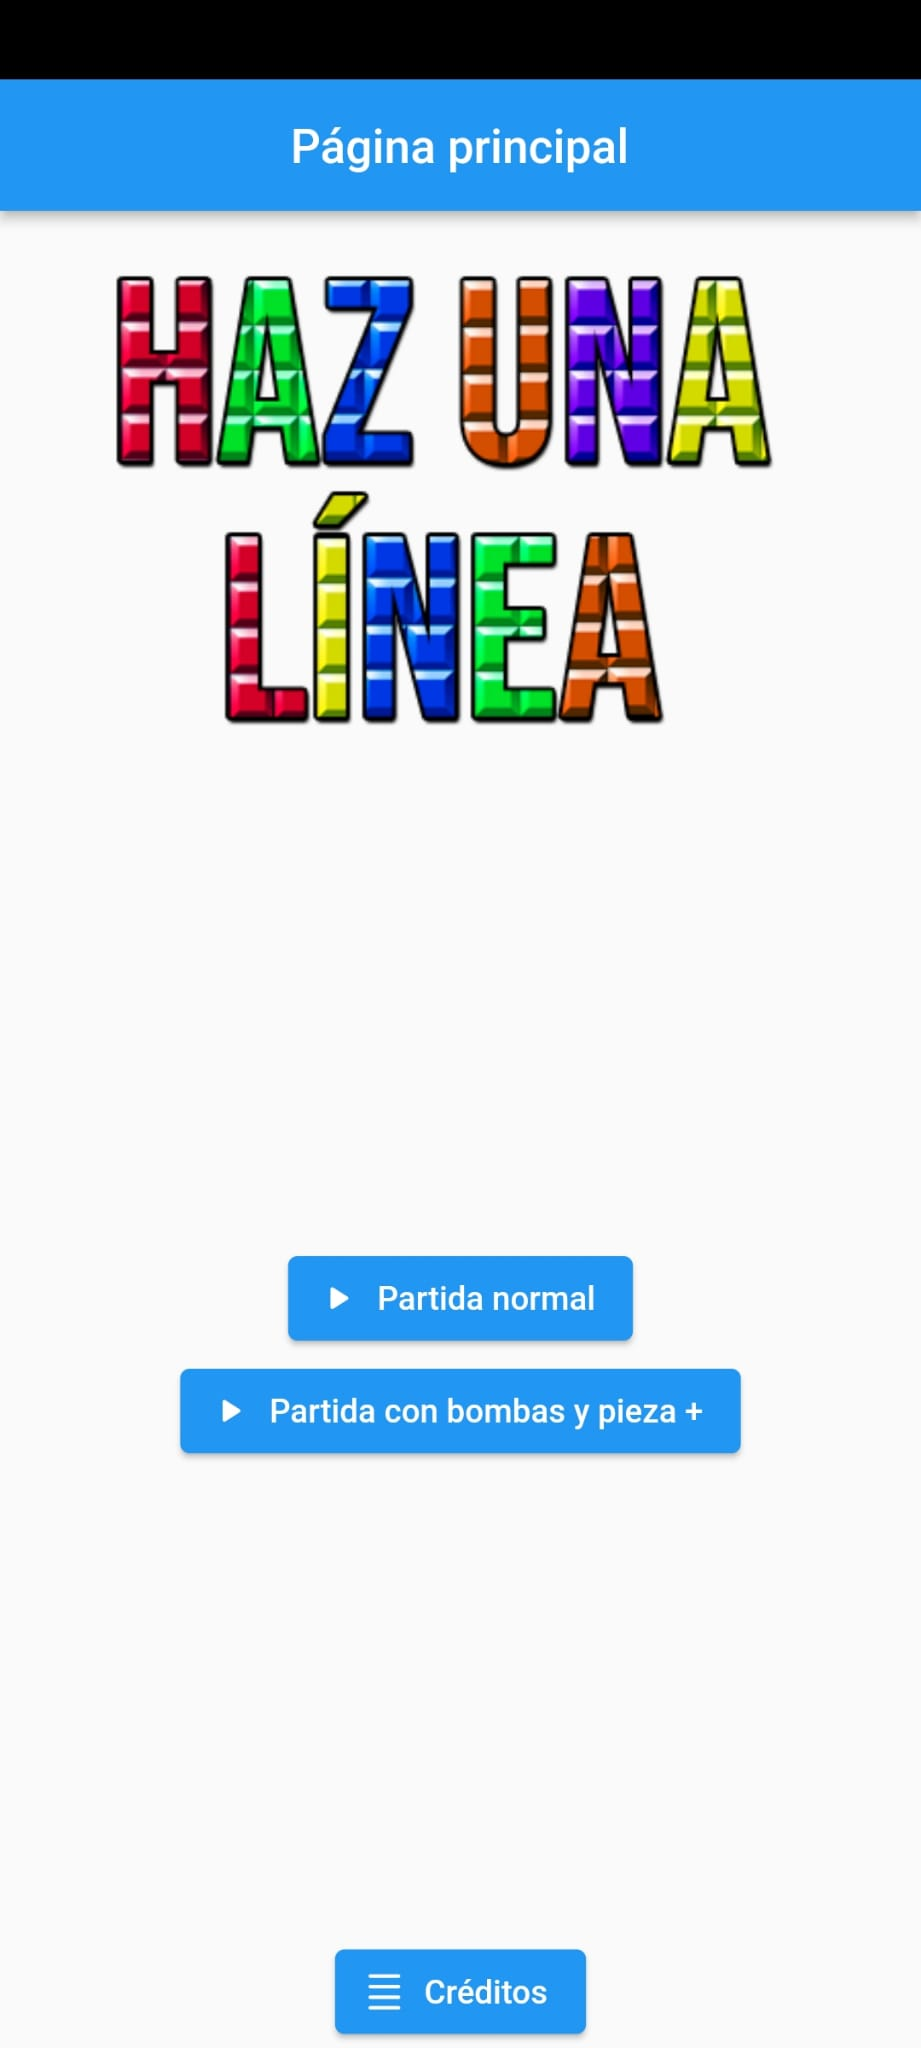
\includegraphics[scale=0.28]{imagenes/captura7.jpeg}
        \caption{Pantalla de inicio de la aplicación}
\end{figure}

\begin{figure}[H]
\center
        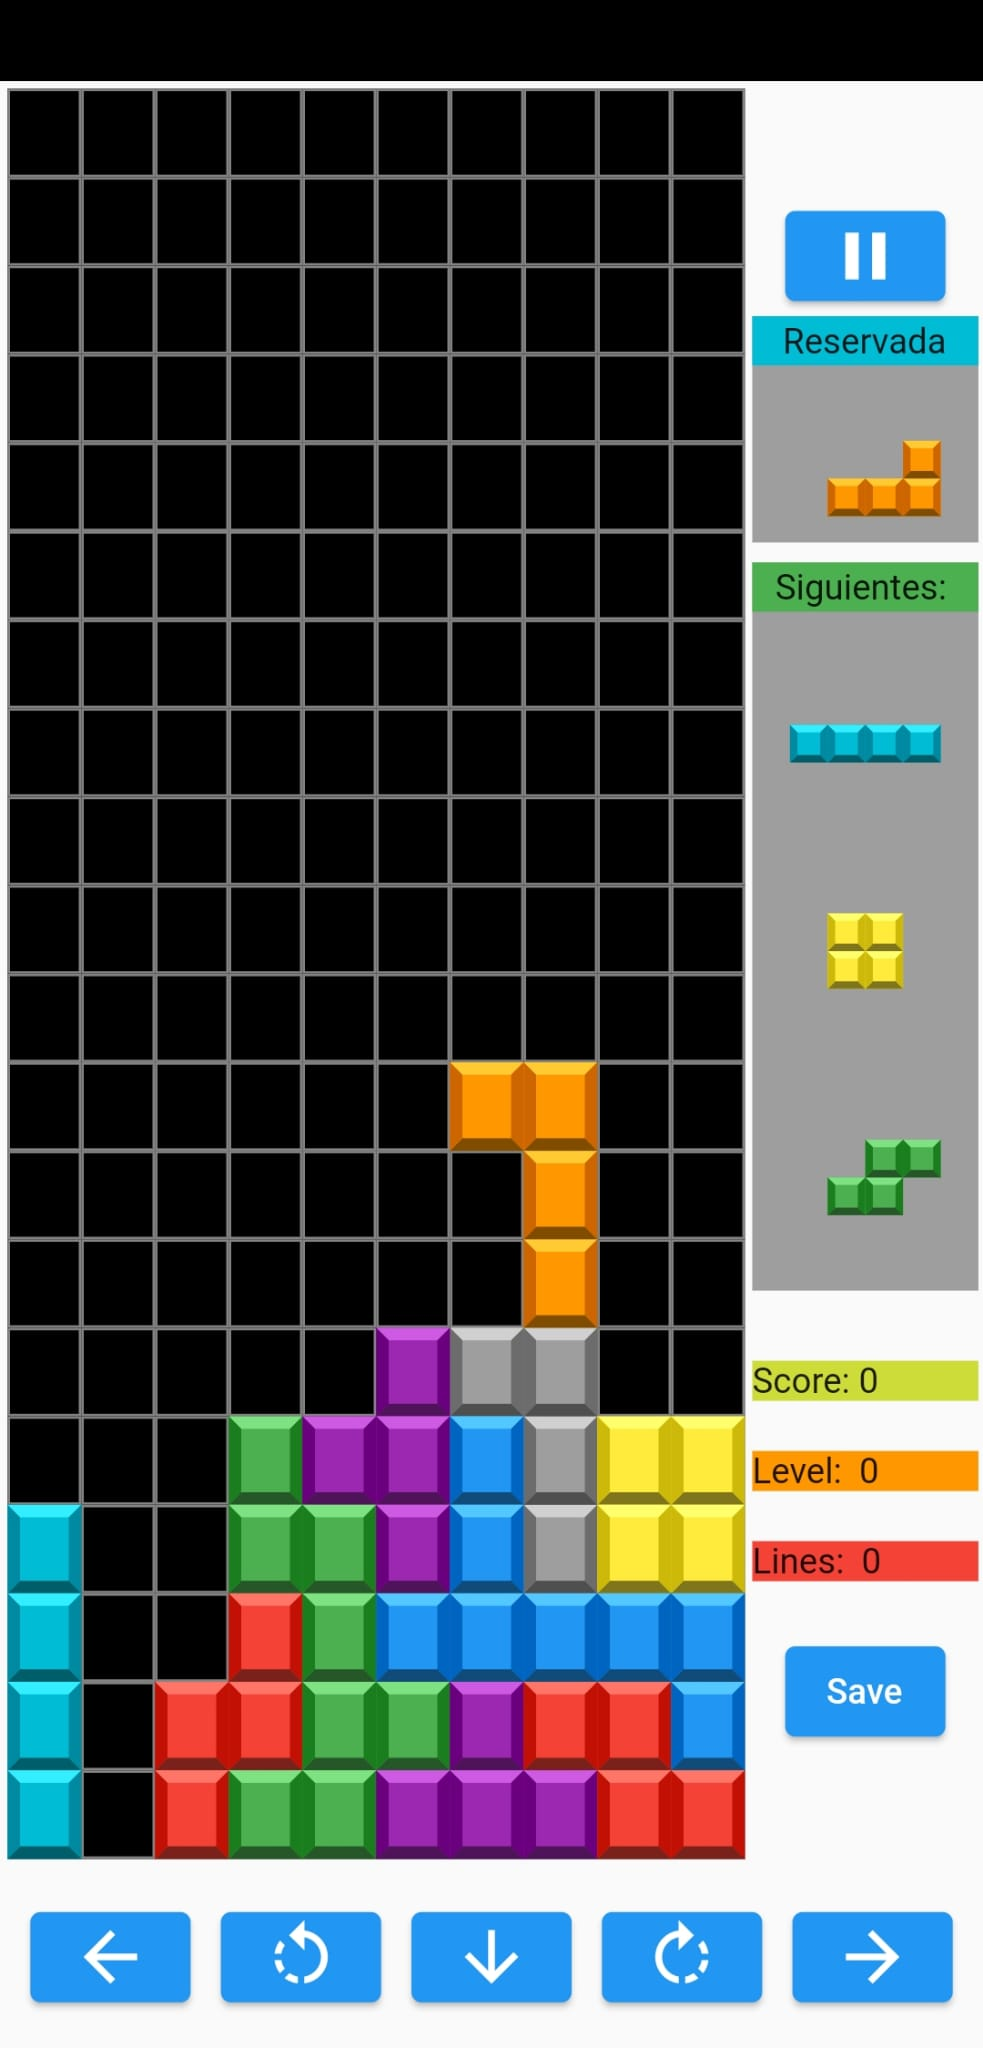
\includegraphics[scale=0.3]{imagenes/captura1.jpeg}
        \caption{Ejemplo de tablero}
\end{figure}

\begin{figure}[H]
\center
        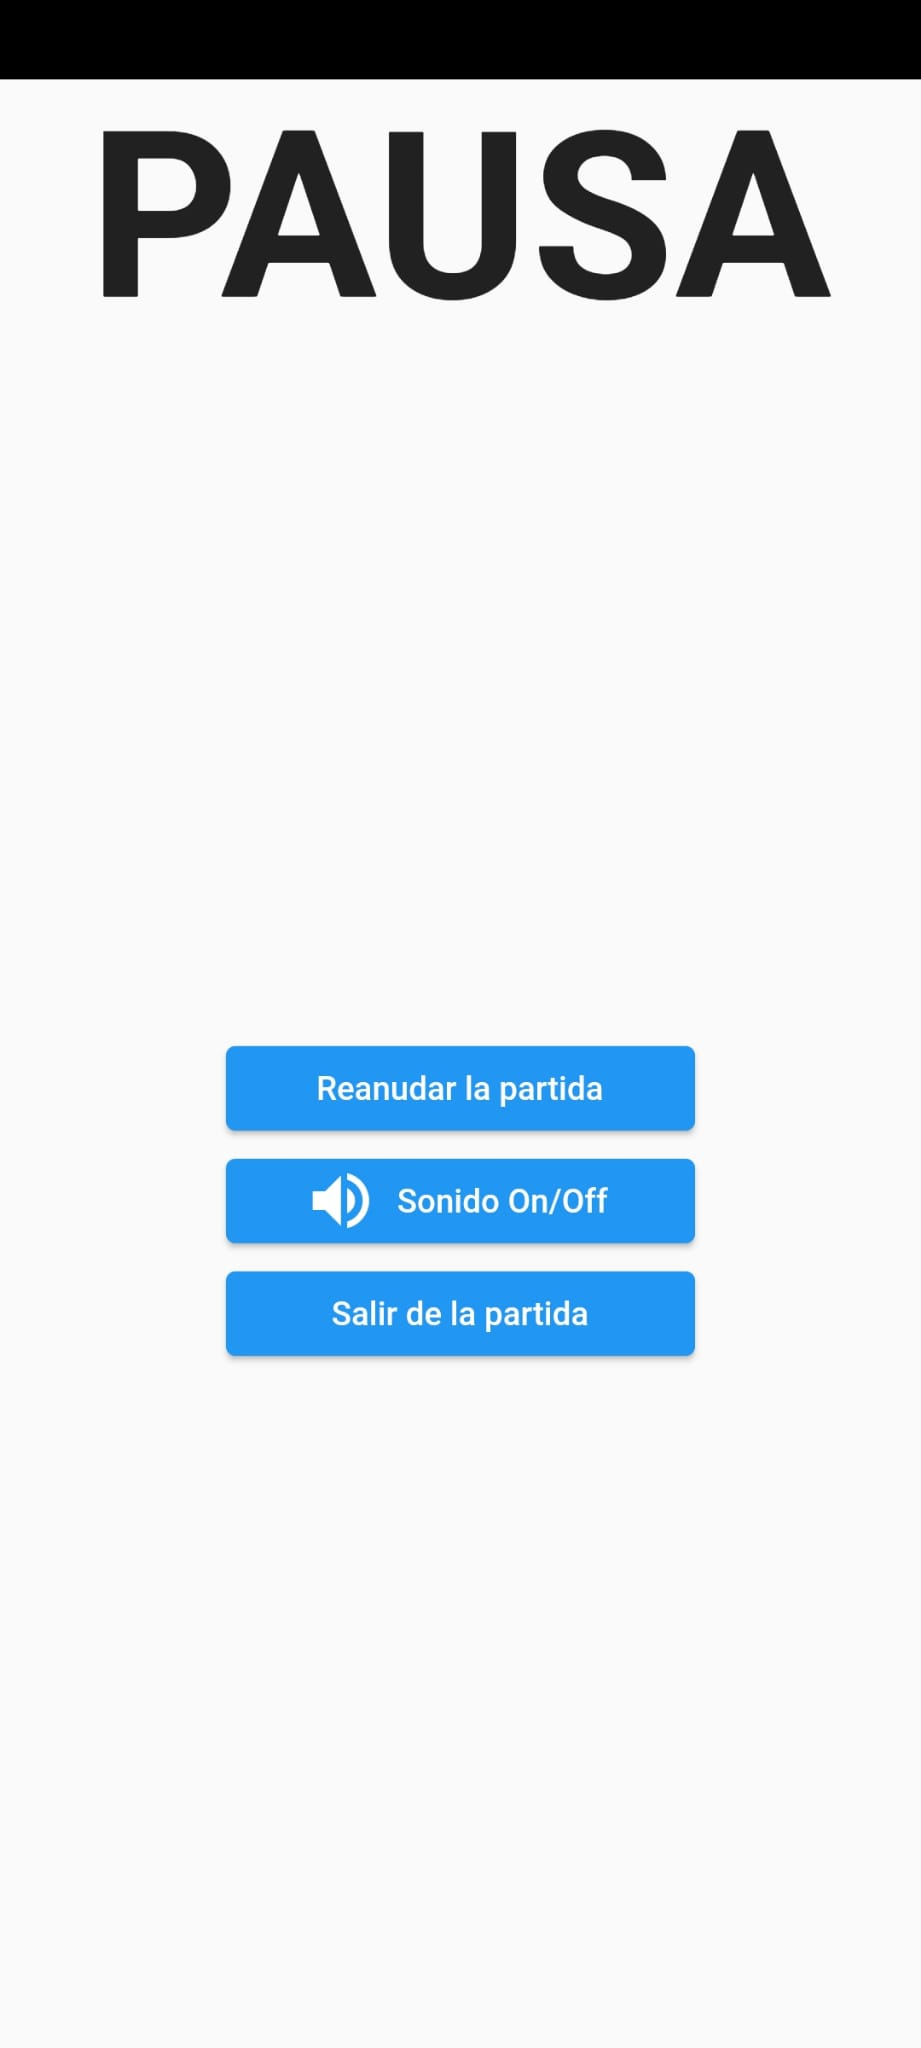
\includegraphics[scale=0.3]{imagenes/captura6.jpeg}
        \caption{Pausa del juego}
\end{figure}

\begin{figure}[H]
\center
        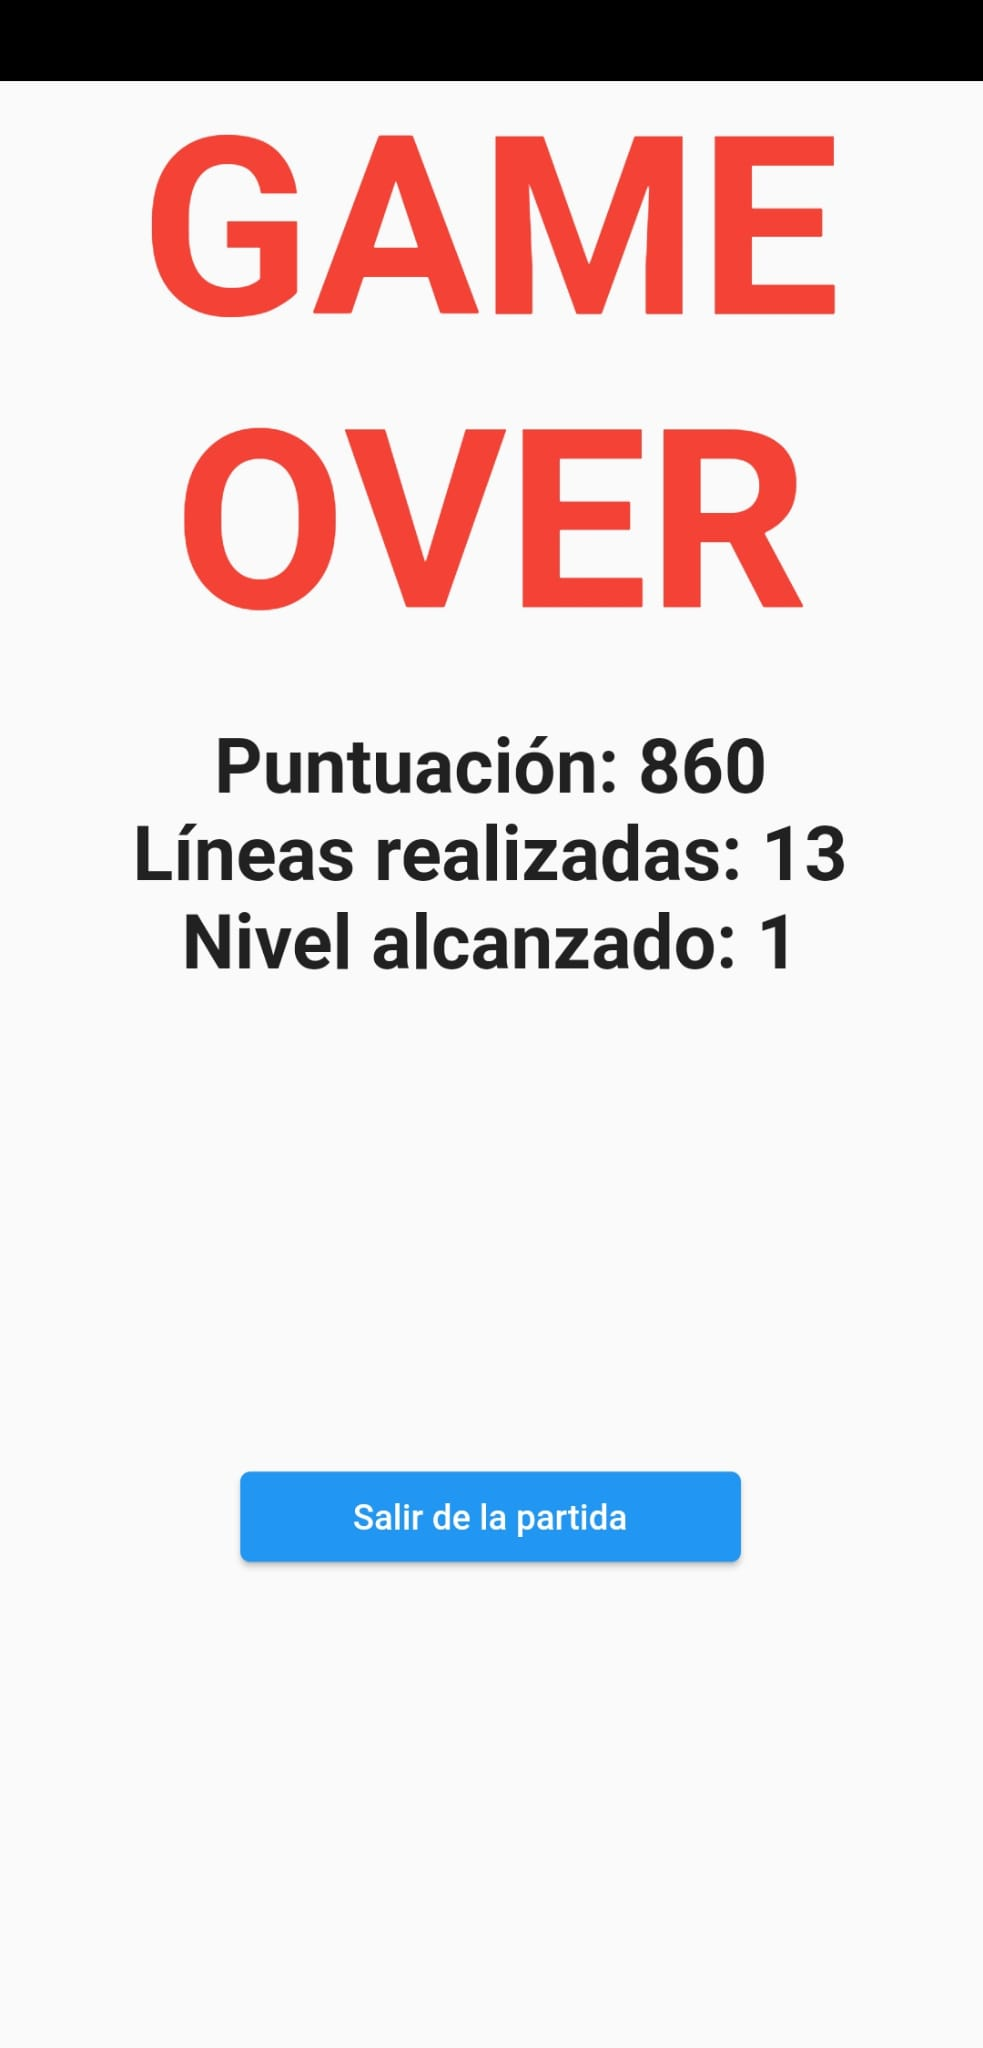
\includegraphics[scale=0.3]{imagenes/captura4.jpeg}
        \caption{Pantalla de Game Over}
\end{figure}

\begin{figure}[H]
\center
        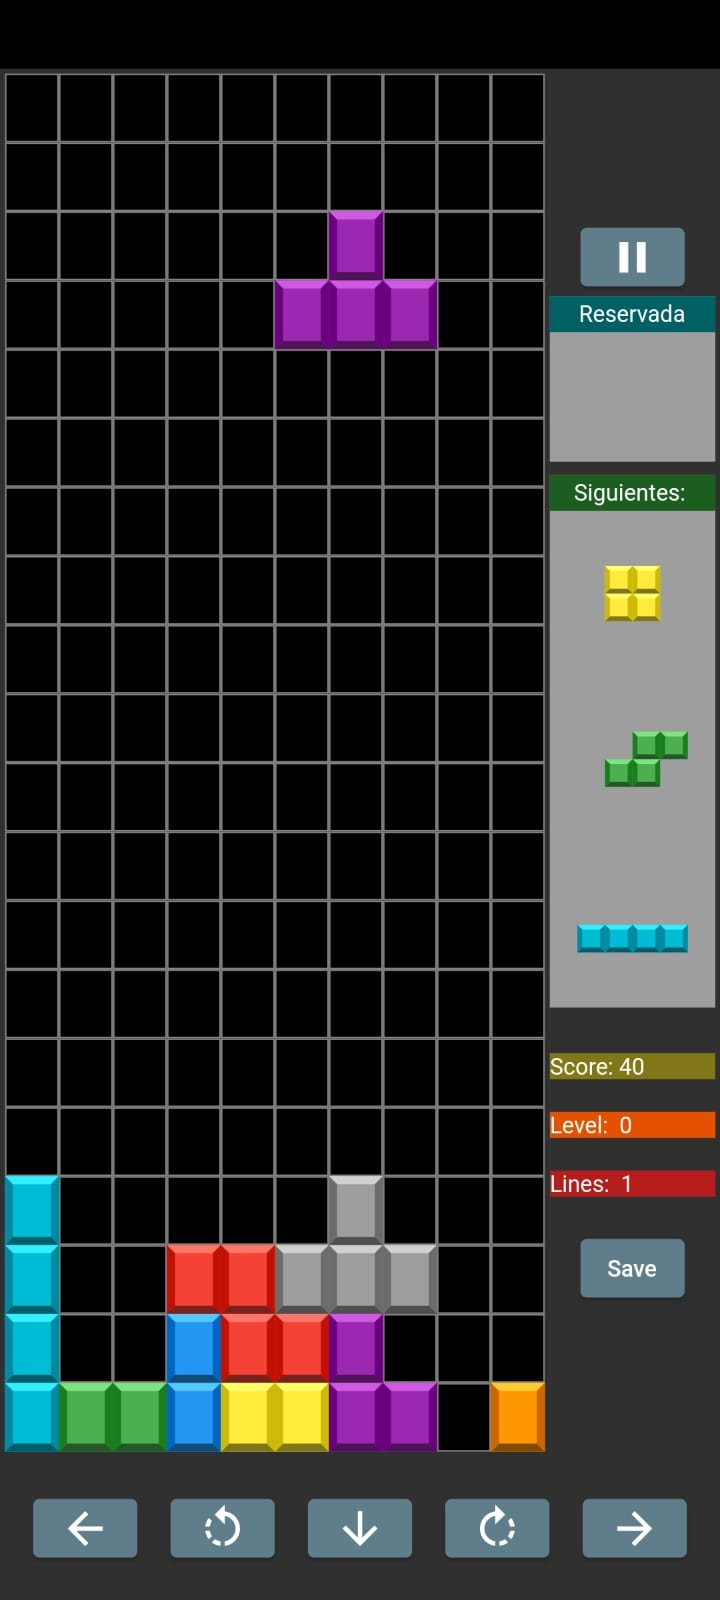
\includegraphics[scale=0.4]{imagenes/captura2dark.jpeg}
        \caption{Modo oscuro de la aplicación}
\end{figure}


\end{document}
